

\documentclass{beamer}
 
\usepackage[utf8]{inputenc}
 \usetheme{Madrid}
 \usecolortheme{beaver}
 \usefonttheme{structuresmallcapsserif}
 \usepackage{listings}
%Information to be included in the title page:


\title[Distributed Systems] %optional
{Naming}

\subtitle{An Overview}

\author[Dr. Joseph Kehoe] % (optional, for multiple authors)
{Joseph Kehoe\inst{1}}

\institute[IT Carlow] % (optional)
{
	\inst{1}%
	Department of Computing and Networking\\
	Institute of Technology Carlow
}

\date[ITC 2018] % (optional)
{CDD101, 2018}

\logo{
\includegraphics[height=1.5cm]{../../itcarlowlogo.png}}




 
 \AtBeginSection[]
 {
 	\begin{frame}
 		\frametitle{Table of Contents}
 		\tableofcontents[currentsection]
 	\end{frame}
 }
 
 
 
\begin{document}
 
\frame{\titlepage}
 
  \begin{frame}
  	\frametitle{Table of Contents}
  	\tableofcontents
  \end{frame}
 

\section{Naming}
  \begin{frame}
  	\frametitle{Introduction}

  	\begin{itemize}
  		\item A string of bits or characters refering to an entity
  		\item An entity can be many things e.g. Printer, Server, file, disk, user, etc.
  		\item Entities can be acted on (through an interface)
  		\item Therefore they have access points
  		\item Access points are known as \textbf{addresses} 
  		\item An entity may have more than one access point (e.g. Phone number)
  		\item Entity can change access point over time 
  	\end{itemize}

  	
  		%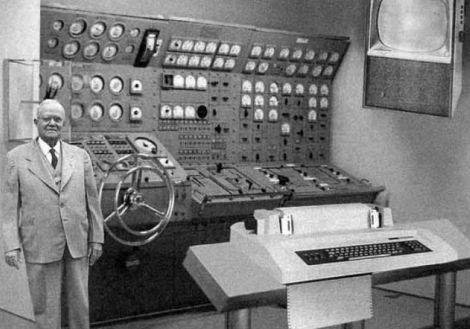
\includegraphics[height=4cm]{Old-Server.jpg}
  \end{frame}
  
    \begin{frame}
    	\frametitle{Identifiers}
    	
    	\begin{itemize}
    		\item Entity name should ideally be independent of its address \textbf{Location Independence}
    		\item Entities need \textbf{Identifiers}
    	\end{itemize}
    	An Identifier has the following properties:
    	\begin{enumerate}
    		\item Refers to at most one entity
    		\item Each entity is refered to by at most one identifier
    		\item An identifier is permanent. It always refers to the same entity (e.g. PPS)
    	\end{enumerate}
    	
    	%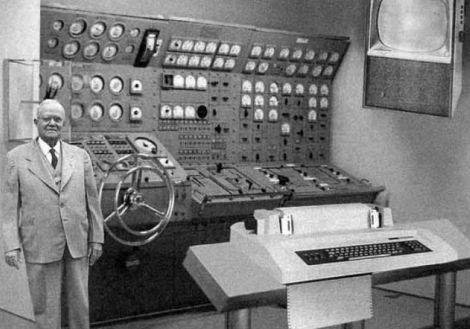
\includegraphics[height=4cm]{Old-Server.jpg}
    \end{frame}
 
    \begin{frame}
    	\frametitle{Name Spaces}
    	
    	\begin{itemize}
    		\item A namespace is a labeled directed graph where:
    		\item Each leaf node refers to an entity
    		\item Non leaf nodes are kown as directory nodes (e.g. Domain Names)
    		\item Absolute path ending in leaf node refers to unique entity
    		\item Relative path ending in leaf node may refer to more than one entity depending on starting point
    		\item Looking up a name is known as \textbf{Name Resolution}
    	\end{itemize}
    	
    	%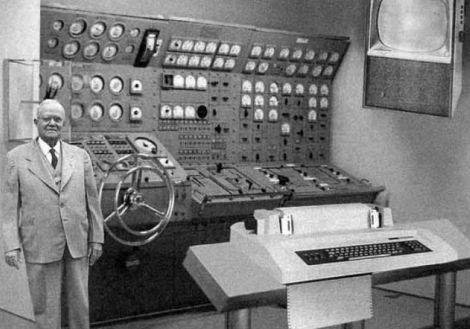
\includegraphics[height=4cm]{Old-Server.jpg}
    \end{frame}
       
    \begin{frame}
    	\frametitle{Name Space Implementation}
    	Name Space graph is divided into three parts:
    	\begin{description}
    		\item[Global Level] Top Level of graph.  Here graph is very static (e.g .edu, .org, .ie in Domain names)
    		\item[Administrative Layer] Middle layer.  Graph is still static in nature, does not change much 
    		\item[Managerial Layer] Lower level. Most likely to change over time
    	\end{description}
    	\begin{itemize}
    		\item Static layers can be cached
    		\item Use high performance and reliable servers (replicated) to run top levels 
    	\end{itemize}
    	%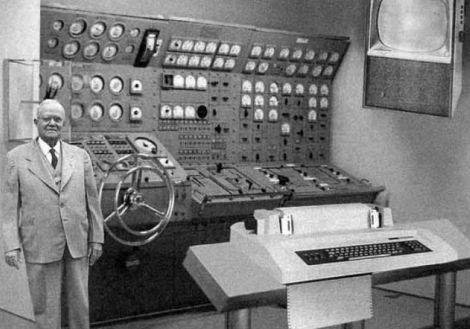
\includegraphics[height=4cm]{Old-Server.jpg}
    \end{frame}
\section{Mobility}
    \begin{frame}
    	\frametitle{Locating Mobile Entities}
    	\begin{itemize}
    		\item Allowing mobility for entities creates problems for naming
    		\item use of identifiers helps (seperates naming from location)
    		\item Identifiers tend not to be human friendly
    		\item A location service is used to locate entities
    	\end{itemize}

    \end{frame}
    \begin{frame}
    	\frametitle{Mobile Entity Solutions}
    	Many different approaches to handling mobile entities. All have issues.
    	\begin{description}
    		\item [Broadcast-Multicast] Broadcast identifier to all and wait for response from current "location"
    		\item [Forwarding Pointers] When entity moves old reference keeps pointer to new location forming chains of pointers to entity
    		\item[Home Based Approach] Original location of enity is the home location. This always keeps track of current location of entity
    		\item[Hierarchical Approach] Similar to DNS. Caching can help here if entities are not highly(?) mobile
    	\end{description}
    	
    \end{frame}    
    
\section{Referencing}
    \begin{frame}
    	\frametitle{Removing Unreferenced Entities}
    	Similar to garbage collection for pointers but much worse
    	\begin{itemize}
    		\item How do we track references to an entity when those references come from many distributed machines?
    		\item Reference counting helps but we must count across machines
    		\item \textbf{Weighted Reference counting} helps. But it still has issues
    		\item \textbf{Reference listing} is where each skeleton keeps a list of every proxy that links to it (Java RMI)
    	\end{itemize}
    	
    \end{frame} 

\end{document}

